\section{Casi d'Uso}\label{CasiUso}
\subsection{Introduzione}\label{CasiUso_Introduzione}
Nella seguente sezione verranno identificati i casi d'uso individuati dal team \texttt{Agents of S.W.E.}.\\
Il numero di casi analizzati è limitato poiché il plug-in fornisce funzionalità aggiuntive ad una piattaforma preesistente, per la quale non è fornita documentazione in quanto già disponibile presso il sito web del fornitore della piattaforma: \href{http://docs.grafana.org/}{\textit{Grafana Labs}}.\\

\subsection{Attori}
\subsubsection{Attori primari}


\subsubsection{Attori secondari}

\subsection{Elenco dei casi d'uso}

%\begin{itemize}
%\item \textbf{Attore primario:}
%\item \textbf{Precondizioni:}
% \begin{enumerate}
% \item
% \end{enumerate}
%\item \textbf{Postcondizioni:}
% \begin{enumerate}
% \item
% \end{enumerate}
%\item \textbf{Scenario Principale:}
% \begin{enumerate}
% \item
% \end{enumerate}
%\item \textbf{Estensioni:}
%\end{itemize}

\subsubsection{UC1 - Aggiunta della rete bayesiana al plug-in G\&B}\label{UC1}
\begin{itemize}
	\item \textbf{Attore primario}: Utente registrato;
	\item \textbf{Precondizioni}: l'utente deve aver effettuato il login nella piattaforma Grafana, deve aver selezionato una Dashboard e aggiunto il pannello "G\&B Panel".
	\item \textbf{Postcondizioni}: l'utente ha aggiunto la rete bayesiana al plug-in. Attraverso UC2 (§\ref{UC2}) può selezionare quali nodi sorgente collegare alla rete.
	\item \textbf{Scenario principale:}
	\begin{enumerate}
		\item L'utente accede alla piattaforma Grafana, si trova nella dashboard preferita ed ha aggiunto il pannello "G\&B Panel";
		\item L'utente seleziona e clicca sul bottone con simbolo di "+" (UC1.1, §\ref{UC1.1});
		\item L'utente si trova davanti una finestra presso cui selezionare il file JSON contenente la rete (UC1.2, §\ref{UC1.2}) e seleziona "Aggiungi".
	\end{enumerate}
\end{itemize}

\subsubsection{UC1.1 - Apertura pannello di selezione della rete bayesiana}\label{UC1.1}
\begin{itemize}
	\item \textbf{Attore primario}: Utente registrato; 
	\item \textbf{Precondizioni}: l'utente visualizza il pannello "G\&B Panel" nella dashboard.
	\item \textbf{Postcondizioni}: l'utente ha cliccato il bottone con etichetta "+" e visualizza il pannello per la selezione del file della rete.
	\item \textbf{Scenario principale:} l'utente seleziona clicca il pulsante con etichetta "+" nel pannello "G\&B Panel" nella dashboard.
\end{itemize}


\subsubsection{UC1.2 - Selezione della rete bayesiana}\label{UC1.2}
\begin{itemize}
	\item \textbf{Attore primario}: Utente registrato;
	\item \textbf{Precondizioni}: l'utente ha cliccato il bottone con etichetta "+".
	\item \textbf{Postcondizioni}: l'utente ha selezionato la rete bayesiana desiderata e ha premuto il pulsante con etichetta "Aggiungi".
	\item \textbf{Scenario principale:}
	\begin{enumerate}
		\item L'utente seleziona dalla finestra il file da importare;
		\item L'utente clicca il pulsante con etichetta "Aggiungi".
	\end{enumerate}
	\item \textbf{Estensioni}:
	\begin{itemize}
		\item \hyperref[UC6]{UC6 (\ref*{UC6})} La mappa selezionata non è corretta per estensione o per contenuto;
		\begin{enumerate}
			\item L'aggiunta della rete al plug-in fallisce;
			\item Viene visualizzato un messaggio di errore esplicito che spieghi l'errore;
			\item Viene fornita all'utente un'altra possibilità per selezionare il file corretto.
		\end{enumerate}
	\end{itemize}
\end{itemize}

\begin{figure}[h!]
	\begin{center}
		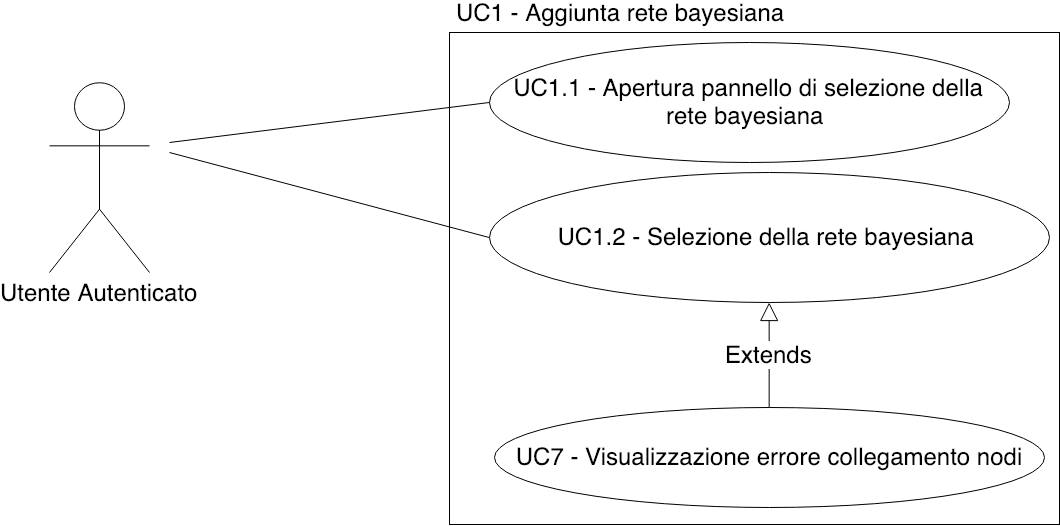
\includegraphics[scale=0.5]{./images/UC1.png}
		 \caption{Rappresentazione di UC1.}	
	\end{center}
\end{figure}

\pagebreak

\subsubsection{UC2 - Collegamento nodi al flusso dati}\label{UC2}

\begin{figure}[H]
\centering
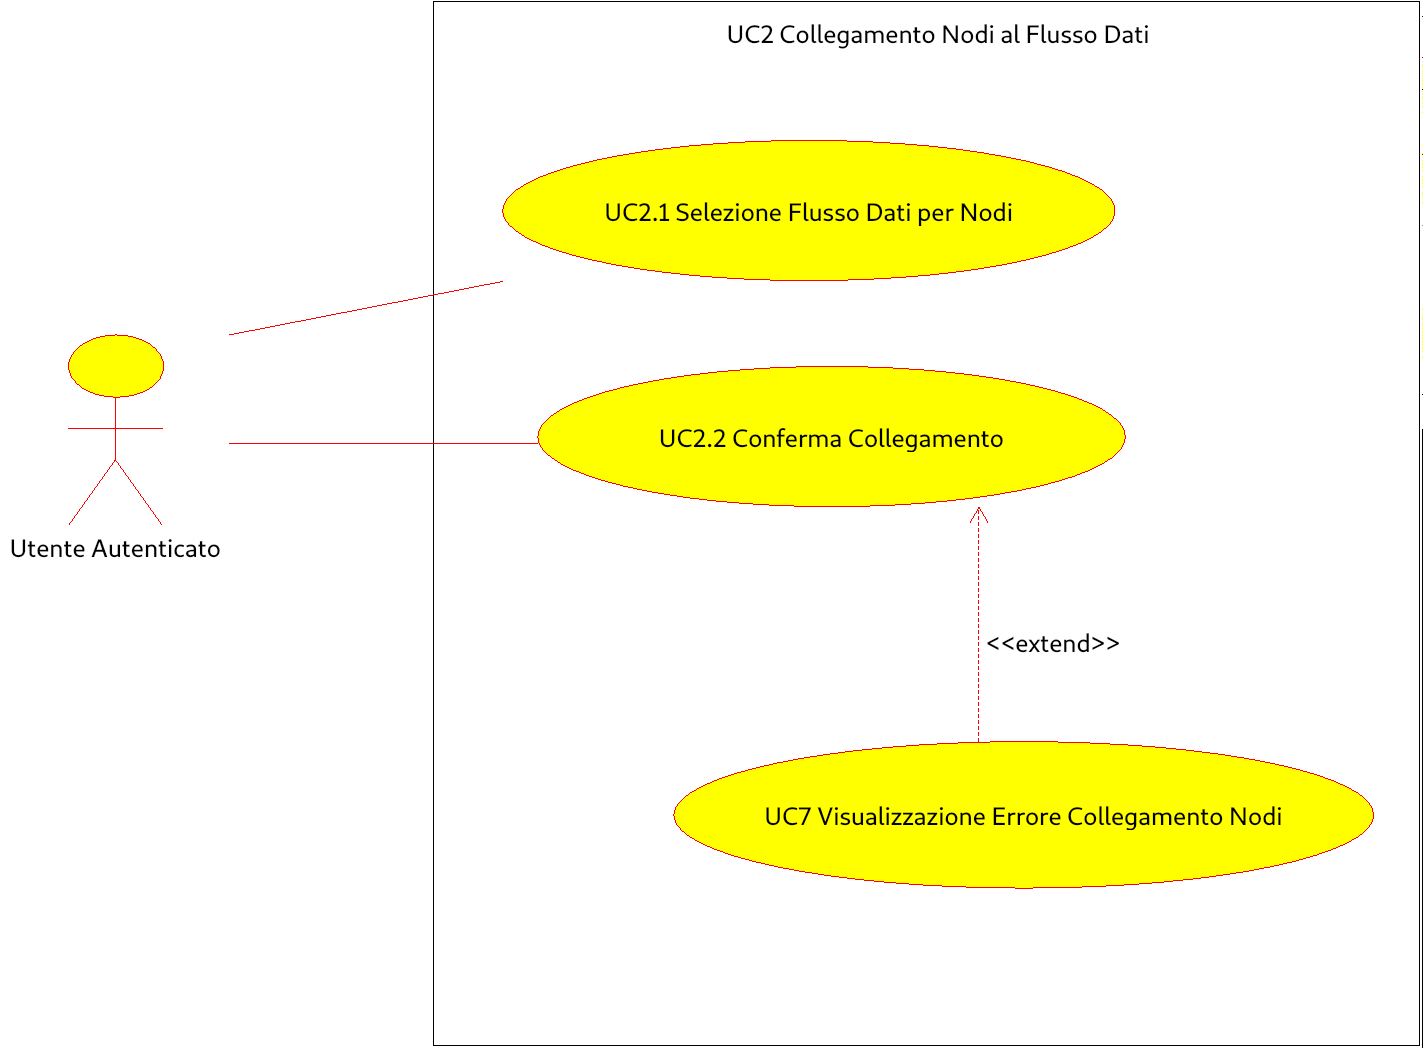
\includegraphics[scale=0.3]{./images/UC2.png}
\caption{UC2 - Collegamento nodi della rete bayesiana al flusso dati}
\end{figure}

\begin{itemize}
\item \textbf{Attore primario:} Utente Autenticato;
\item \textbf{Precondizione:} L'utente ha caricato con successo la rete bayesiana (\hyperref[UC1]{UC1 (\ref*{UC1})});
\item \textbf{Postcondizione:} L'utente ha collegato con successo i nodi desiderati della rete bayesiana caricata in \hyperref[UC1]{UC1 (\ref*{UC1})};
\item \textbf{Scenario principale:}
	\begin{enumerate}
	\item L'utente collega i nodi desiderati ad un flusso dati (\hyperref[UC2.1]{UC2.1 (\ref*{UC2.1})});
	\item L'utente conferma il collegamento dei nodi (\hyperref[2.2]{UC2.2 (\ref*{UC2.2})}).
	\end{enumerate}
\item \textbf{Estensioni:} \hyperref[UC7]{UC7 (\ref*{UC7})} estende \hyperref[UC2.2]{UC2.2 (\ref*{UC2.2})}: L'utente visualizza un messaggio di errore nel caso in cui non abbia collegato alcun nodo al flusso dati.
\end{itemize}

\paragraph{UC2.1 - Selezione flusso di dati per ogni nodo}\label{UC2.1}
\begin{itemize}
\item \textbf{Attore primario:} Utente Autenticato;
\item \textbf{Precondizione:} L'utente ha caricato con successo la rete bayesiana (\hyperref[UC1]{UC1 (\ref*{UC1})}).
\item \textbf{Postcondizione:} L'utente ha selezionato il flusso dati opportuno per ogni nodo che desidera collegare alla rete bayesiana.
\item \textbf{Scenario Principale:}
 \begin{enumerate}
 \item L'utente seleziona, tramite click, la checkbox corrispondente al nodo che desidera collegare ad un determinato flusso dati;
 \item L'utente visualizza, a seguito del click precedente, una tendina a comparsa contente i possibili flussi dati a cui collegare il nodo;
 \item L'utente seleziona, tramite click, il flusso dati opportuno a cui collegare il nodo selezionato in precedenza.
 \end{enumerate}
\end{itemize}

\paragraph{UC2.2 - Conferma collegamento}\label{UC2.2}
\begin{itemize}
\item \textbf{Attore primario:} Utente Autenticato;
\item \textbf{Precondizione:} L'utente ha caricato con successo la rete bayesiana (\hyperref[UC1]{UC1 (\ref*{UC1})});
\item \textbf{Postcondizione:} L'utente ha collegato con successo i nodi desiderati, della rete bayesiana caricata in \hyperref[UC1]{UC1 (\ref*{UC1})}, ai rispettivi flussi dati;
\item \textbf{Scenario Principale:} L'utente conferma le proprie scelte (\hyperref[UC2.1]{UC2.1 (\ref*{UC2.1})}) cliccando il pulsante "Conferma";
\item \textbf{Estensioni:} \hyperref[UC7]{UC7 (\ref*{UC7})}: L'utente visualizza un messaggio di errore nel caso in cui non abbia collegato alcun nodo al flusso dati.
\end{itemize}

\pagebreak

\subsubsection{UC3 - Politiche temporali di ricalcolo delle probabilità}\label{UC3}

\pagebreak

\subsubsection{UC4 - Visualizzazione dati forniti dai nodi non collegati al flusso}\label{UC4}

\begin{figure}[H]
\centering
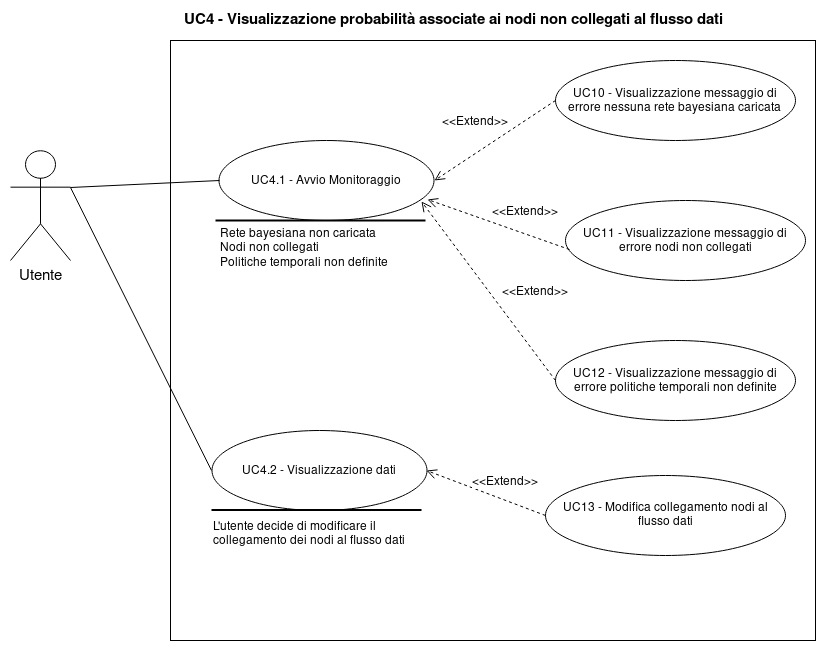
\includegraphics[scale=0.4]{./images/UC4.png}
\caption{UC4 - Visualizzazione dei dati forniti dai nodi non collegati al flusso}
\end{figure}

\begin{itemize}
\item \textbf{Attore primario:} Utente Autenticato;
\item \textbf{Precondizioni:}
	\begin{enumerate}
	\item L'utente ha collegato con successo alcuni nodi della rete bayesiana al flusso dati (\hyperref[UC2]{UC2 (\ref*{UC2})});
	\item L'utente ha definito le politiche temporali per il ricalcolo delle probabilità relative ai nodi della rete bayesiana (\hyperref[UC3]{UC3 (\ref*{UC3})}).
	\end{enumerate}
\item \textbf{Postcondizione:} L'utente visualizza i dati forniti dai nodi della rete bayesiana non collegati al flusso;
\item \textbf{Scenario Principale:} L'utente visualizza le probabilità associate ad ogni nodo della rete bayesiana non collegato al flusso dati (\hyperref[UC2]{UC2 (\ref*{UC2})}). Tali probabilità vengono ricalcolate, e dunque mutano dinamicamente, in base alle politiche temporali stabilite in \hyperref[UC3]{UC3 (\ref*{UC3})}.
\end{itemize}

\pagebreak

\subsubsection{UC5 - ...}\label{UC5}

\subsubsection{UC6 - ...}\label{UC6}

\subsubsection{UC7 - Visualizzazione messaggio di errore collegamento nodi}\label{UC7}
\begin{itemize}
\item \textbf{Attore primario:} Utente Autenticato;
\item \textbf{Precondizione:} L'utente ha confermato il collegamento dei nodi al flusso dati (\hyperref[UC2.2]{UC2.2 (\ref*{UC2.2})}) senza averne effettivamente collegato alcuno;
\item \textbf{Postcondizione:} L'utente visualizza l'errore;
\item \textbf{Scenario Principale:} L'utente visualizza un messaggio di errore in cui è segnalato il fatto che non è stato collegato alcun nodo al flusso dati durante \hyperref[UC2]{UC2 (\ref*{UC2})}.
\end{itemize}
